\subsection{Laboratoire universitaire des sciences appliquées de Cherbourg (LUSAC)}

Dans le contexte de mon stage, l'entreprise qui m'a recruté pour cette expérience professionnelle est LUSAC.\\


\begin{figure}[H]
	\centering
	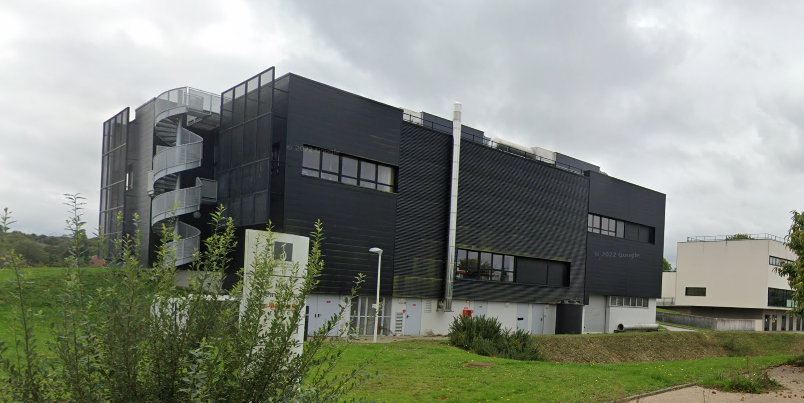
\includegraphics[height=4in]{./IMAGES/LUSACB.png}
	\captionsetup{font=small} 
	\caption[Bâtiment LUSAC]{Bâtiment du LUSAC. ( \href{https://www.google.com/maps/@49.6335523,-1.6514845,3a,75y,226.26h,90.33t,357.47r/data=!3m6!1e1!3m4!1sF4kSy9GKBnB_wiRnWqLzZw!2e0!7i16384!8i8192?hl=fr&entry=ttu}{Google map - Site du LUSAC})}


	\label{fig:LUSAC}

\end{figure}



LUSAC(EA 4253), pour Laboratoire Universitaire des Sciences Appliquées de Cherbourg, a été fondé en 1994 (\cite{LUSAC}) C'est un centre de recherche renommé et dynamique situé à Cherbourg, en France. Il s'agit d'une composante importante de l'Université de Caen Normandie, consacrée à l'innovation et aux découvertes dans le champ des sciences appliquées.

Ce laboratoire a été établi dans le but principal de promouvoir les avancées scientifiques et technologiques par le biais de la recherche de pointe et du développement collaboratif.


Les opérations du laboratoire sont orientées autour de deux axes majeurs : la recherche fondamentale et la recherche appliquée. La première vise à élargir notre compréhension des sciences appliquées, tandis que la seconde s'efforce d'exploiter ces connaissances pour résoudre des défis pratiques et répondre aux exigences de l'industrie.

Depuis son inauguration, le LUSAC a introduit plusieurs innovations technologiques et a participé à de nombreux projets pour la recherche, ce qui témoigne de son dévouement à l'expérience scientifique de haute qualité et au développement technologique.\\

L’unité de recherche est organisée actuellement autour de trois équipes :\\ « Efficacité Énergétique et Transferts
Thermiques » (EffiTherm ),\\ « Stockage de l’énergie
électrique et matériaux » (SEEM) ,\\ « Écoulements et Environnement » (EE).\\
C'est au sein de cette troisième équipe, dans les locaux de INTECHMER que j'ai effectué mon stage.


\subsection{INTECHMER}
\vspace{.5cm}

L'Institut National des Sciences et Techniques de la Mer (INTECHMER), une institution prestigieuse affiliée au Conservatoire National des Arts et Métiers (CNAM), est situé à Cherbourg, en Normandie. L'INTECHMER est reconnu pour son expertise dans les sciences et techniques maritimes, et s'engage à fournir un enseignement supérieur de haute qualité, combinant théorie et pratique, dans divers domaines liés à la mer.

L'INTECHMER propose trois diplômes distincts :

Cadre Technique Production et Valorisation des Ressources Marines : Cette formation prépare les étudiants à être rapidement opérationnels dans les domaines de la production et de la valorisation des ressources biologiques de l'océan. Les domaines d'application comprennent l'halieutique, l'aquaculture animale et végétale, l'aquariologie, la transformation et la valorisation des produits de la mer, ainsi que les biotechnologies marines.

Bachelor Océanographe - Prospecteur : Cette formation vise à former des cadres techniques dans différents domaines océanographiques appliqués. Les domaines d'application comprennent les énergies marines renouvelables, les travaux sous-marins, la recherche, l'exploration et l'exploitation de ressources minérales marines, le développement de nouvelles techniques de mesure, et la gestion des données océanographiques.

Cadre Technique Génie de l'Environnement Marin : Cette formation pluridisciplinaire prépare des cadres techniques dans les domaines du contrôle, de la surveillance et de la protection du milieu marin. Les domaines d'application comprennent le contrôle de la qualité des eaux, les études d'impact des activités humaines sur l'environnement et les écosystèmes marins, la protection et l'aménagement du littoral, la préservation et la restauration des écosystèmes marins, et la lutte contre la pollution.

\vspace{1.5cm}
\begin{figure}[H]
	\centering
	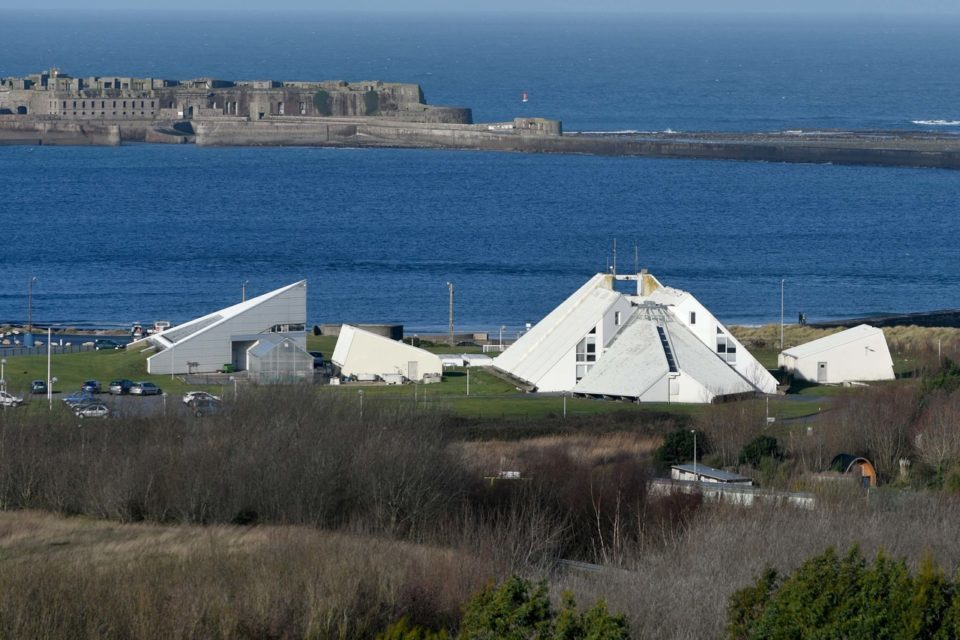
\includegraphics[height=3.5in]{./IMAGES/INtechmer.jpg}
	\captionsetup{font=small} 
	\caption[Bâtiment INTECHMER]{Bâtiment INTECHMER. ( \href{https://actu.fr/normandie/valognes_50615/cherbourg-12-millions-d-euros-pour-renover-l-intechmer_36657872.html}{actu.fr - Normandie})}
	
	
	\label{fig:CNAM}
	
\end{figure}
\vspace{.5cm}
En plus de son engagement en matière d'enseignement, INTECHMER, qui fait partie de l'équipe Écoulement et Environnement de LUSAC, mène également des recherches fondamentales de pointe. Ces recherches visent à approfondir notre compréhension des phénomènes marins et à développer de nouvelles technologies et méthodes pour l'étude et la gestion de l'environnement marin. L'institut joue également un rôle actif dans la diffusion de la culture scientifique et technique, en partageant les résultats de ses recherches avec la communauté scientifique et le public plus large (\cite{CNAM}).

Le pôle de recherche de INTECHMER est organisé autour de trois domaines clés : la sédimentologie, la biologie et l'hydrologie. Ces domaines, bien que distincts, sont interconnectés et nécessitent une approche intégrée pour aborder les problématiques complexes liées à l'environnement marin.

Malgré la diversité de ces thématiques, INTECHMER, en tant que partie intégrante de l'équipe Écoulement et Environnement de LUSAC, utilise une approche interdisciplinaire pour aborder et résoudre des problématiques complexes. En combinant les connaissances et les compétences de différents domaines, INTECHMER est capable d'obtenir des solutions plus complètes et innovantes.

Cette approche interdisciplinaire est un élément clé de la stratégie de recherche de INTECHMER. Elle permet non seulement de résoudre des problèmes complexes, mais aussi de stimuler l'innovation et de favoriser l'excellence en recherche.



\begin{figure}[H]
	\centering
	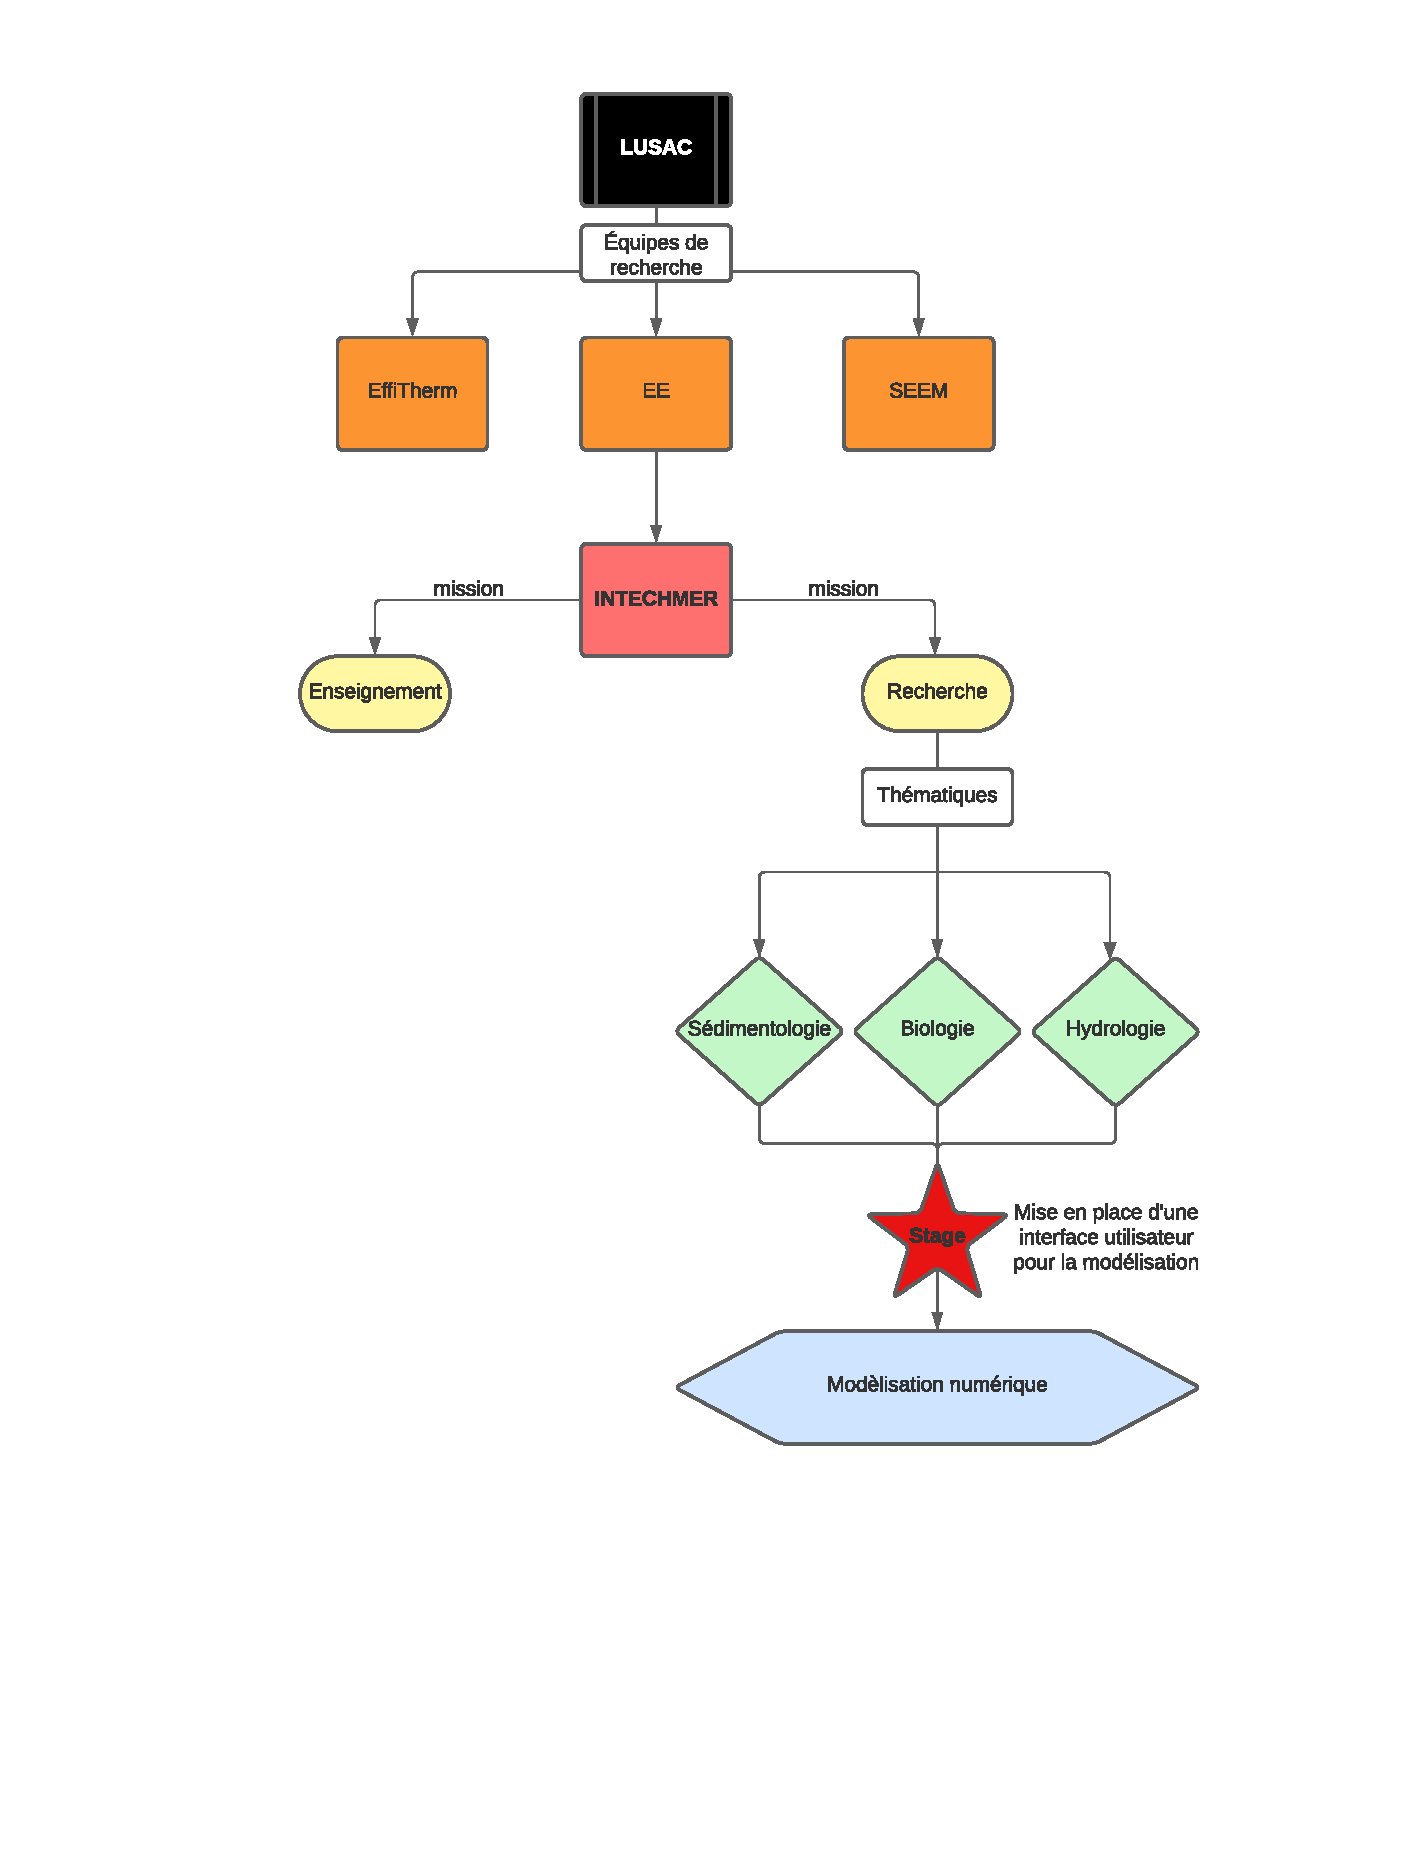
\includegraphics[height=10in]{./IMAGES/histostage.pdf}
	\captionsetup{font=small} 
	\caption[Contexte Stage.]{Contexte Stage. ( {Récapitulatif de la place du stage au sein de l'entreprise})}
	
	
	\label{fig:Stage}
	
\end{figure}